\chapter{Introduction}\label{chapter:introduction}
Cancer remains one of the most formidable challenges in the realm of health and medicine, causing a quarter of all deaths in the UK \cite{noauthor_cancer_2015}.
Despite advances in cancer research, the survival rates for many cancers remain low, with the disease being an increasing burden on healthcare
systems \cite{noauthor_financial_nodate}. The disease's heterogeneity, both within and between patients, is a major obstacle to effective treatment. Understanding the
underlying evolutionary processes driving this heterogeneity is crucial to developing new treatments and improving patient outcomes.
While having a comprehensive mathematical theory of cancer evolution may not be feasible, concrete mathematical models can provide valuable insights into the
disease's dynamics. To this end, we consider different approaches to modelling cancer evolution via driver mutations, which includes the use of phylogenetic
trees and agent-based models. Further, we employ methylation data to verify the accuracy of our models using Approximate Bayesian Computation (ABC).\par
Trees as a mathematical object have found use in a variety of fields, of which biology is our main focus. However, while writing this thesis, we have found
treesinteresting links to methods in computer science via information theory.
In chapter \ref{chapter:trees}, we expand upon three points. First, we further establish $J^1$ as a
universal index of tree balance by identifying funamental connections to classical results in
computer science, related to Huffman coding and self-balancing tree data structures. Second, we derive
upper bounds on the error of the expected value approximations for the Yule process and the uniform models.
For the Yule process, we prove that the approximation rapidly convergest to the true expectation in the
large tree limit. Finally, we investigate the minimal values of $J^1$ in important special cases,
obtaining a counter intuitive result in the large tree limit.\par
In chapter \ref{chapter:trajectories}, we employ the index $J^1$, along with two other tree shape indices, to
test to what degree one can differentiate between different evolutionary regimes in cancer by only relying at
tree shape indices. These results are compared to a new, more comprehensive system of tree shape indices \cite{noble_new_2023}
which further generalised the concepts of diversity, evenness and richness. These results lay the groundwork for
future analysis of cancer tree data.\par
In chapter \ref{chapter:methdemon}, we introduce a proprietary model for simulating a specific type of molecular data, methylation arrays, obtained from
multi-site sequencing of colorectal cancer. We show that the model is able to recapitulate the patterns observed in the
data and that it can be used to infer the evolutionary history of the tumour. We further explore how the model can be expanded
for more general use due to its modular design. We also demonstrate an approximate Bayesian computation workflow for inferring
the parameters of the model from data, and discuss the choice of summary statistics and the performance of the ABC algorithm.\par
In chapter \ref{chapter:methylation}, we use the new agent-based modelling framework to infer the evolutionary history of
$10$ colorectal cancer samples. Additionally, using tree shape indices, we compare trees of the inferred branching process in the data to the trees
generated in the simulation. This provides us an additional tool for validating the model and the inference process. We also
explore the potential of using the model for predicting the future evolution of tumours, and discuss the limitations of the
workflow for our specific use case.\par


\section{Trees and their applications}

\subsection{Introduction}
In the most general sense, a tree is a connected graph with no cycles. In this thesis, when a tree is
mentioned, we refer to a rooted tree, as formally defined in section \ref{sec:preliminary_defs}.
Trees have found use in a variety of fields, including computer science, biology, and linguistics.
In computer science, trees are used to represent hierarchical data structures, such as file systems \cite{nievergelt_binary_1974}
or the structure of a program's syntax \cite{knuth_semantics_1968}, an approach that computer scientists
share with linguists \cite{chomsky_syntactic_1957}. The concept of search trees, dating back to the mid 20th century,
revolutionised the field of computer science with applications in information retrieval in the form of
binary search trees and self-balancing trees \cite{nievergelt_binary_1972, knuth_art_1997}. In biology,
the first appearance of trees dates back to the 19th century, when Charles Darwin used them to represent the evolutionary
relationships between species. Phylogenetic trees have over time become a key tool in analysing the
lineages of species, viral mutations, and cancer evolution. By investigating quantitative summaries of different properties
of tree shapes, we can gain insights into the underlying processes driving the evolution of species \cite{mooers_inferring_1997}
or cancer \cite{scott_inferring_2018, noble_spatial_2022}. However, most of the inference work so far has been performed
using methods which are not necessarily rooted in sound mathematical theory, but are rather based on heuristics \cite{omeara_evolutionary_2012}.
Specifically, measures of tree balance suffer from a lack of a common framework, with at least $19$ different metrics available
in literature \cite{fischer_tree_2021}, and few of them being directly comparable. Also, due to the divergent terminology and
interest in the use of trees as a tool, there is scarce literature on the transfer of knowe=ledge between the fields of computer science
and biology, with certain results being rediscovered nigh on half a century later, as discussed in section \ref{sec:trees_intro}.

\subsection{Quantifying tree balance}
In a recent paper \cite{lemant_robust_2022}, Lemant and Noble proposed a new robust, universal index, $J^1$, for quantifying the
balance of rooted trees with arbitrary node degree and size distributions. This index is based on
Shannon entropy and favours even distributions of node sizes. We showed that $J^1$ is robust, in the sense
that it is insensitive to small changes in node sizes and to the removal of small nodes (figure \ref{fig:robustness}A).
We further showed that this index unites and generalises two of the most
popular prior approaches to quantifying tree balance in biology, the Colless index and the Sackin index.
Applied to evolutionary trees, $J^1$ outperforms conventional tree balance indices as a summary statistic
for comparing model output to empirical data \cite{noble_spatial_2022}.\par
Given any tree shape index, an important task is to obtain its expected and extreme values under standard
tree-generating processes, which can then be used as null-model reference points. In \cite{lemant_robust_2022}, we
obtained analytical approximations to the expected values of $J^1$ under the Yule process and the uniform
model, and tested their accuracy numerically for trees with up to $128$ leaves (figure \ref{fig:robustness}B). In the
same study, we proved that caterpillar trees minimise $J^1$ among bifurcating trees but not when larger
outdegrees are permitted.\par

\begin{figure}
    \centering
    \includegraphics[width=\textwidth]{Chapter_1/figures/ruindices_paper_figures.png}
    \caption{\textbf{a)}} $J^1$ values for $100$ random trees on $16$ leaves using the alpha-gamma model,
    with $\alpha\sim \text{Unif}(0,1)$ and $\gamma\sim \text{Unif}(0,\alpha)$. The values were
    calculated before and after applying a $1\%$ population threshold, i.e. removing all leaves
    with sizes smaller than $0.01$ times the total population. textbf{b)}} $J^1$ values
    for trees generated under the Yule process and the uniform model. Solid curves represent the approximate
    expected values, and the dashed lines the $5$th and $95$th percentiles.\}
    \label{fig:robustness}
\end{figure}


\section{Agent-based modelling in oncology}

\subsection{Introduction}
Agent-based models (ABMs) are a class of computational models that simulate the actions and interactions of individual
agents within a system. These agents can represent anything from cells in a tissue to animals in an ecosystem. ABMs
are particularly useful in cancer research, as they can capture the complex interactions happening on the microscale in
cancer. Spatial agent-based models (SABMs) are a subclass of ABMs that incorporate spatial information into the
simulations. This is particularly useful for modelling solid tumours as it allows for the simulation of things like
the spatial heterogeneity of the tumour microenvironment and the effects of spatial constraints on tumour growth.
A strength of ABMs is that they can be as simple or as complex as the researcher needs them to be \cite{colyer_seven-step_2023}.
However, therein lies their weakness, as oversimplification of a model can lead to rapid loss of its utility in
modelling the behaviour of a complex system such as cancer. On the other hand, a model that is too complex, and
attempts to include everything from epigenetic mutations to the effects of the immune system on the tumour, is likely
too computationally expensive to be useful for modelling a tumour of reasonable size. This is an organic demonstration
of many a researcher's favourite saying \textit{all models are wrong, but some are useful, and some are more useful
than others}. In parsing through the literature and developing a new model of our own, we have also been influenced
by an alternative wording of this, that is \textit{the best model is its own worst enemy}, by Philip Maini. Our
interpretation is that a good model should address the questions it was designed to answer, but also open up new
ones which require further investigation, improvements, and research. For example, one can use our demon-warlock
framework \cite{bak_warlock_2023} to simulate the evolution of a tumour in space and draw conclusions on how
spatial organisation will impact intratumour heterogeneity or patient outcomes \cite{noble_when_2020, noble_spatial_2022}.
However, the model does not address the impact of the immune system, spatial heterogeneity in the microenvironment,
or the effects of therapy without further modifications. Alternatively, we may want to include diffusion of
nutrients and waste products in the model, or the effects of hypoxia on the tumour cells. Tools that would be
appropriate for such tasks are, for example, HAL \cite{bravo_hybrid_2020} or PhysiCell \cite{ghaffarizadeh_physicell_2018},
but they are not ideal either as simulating a realistically-sized tumour with these models is prohibitively expensive
in terms of computational resources. Thus, our preferred approach is to develop a proprietary model which is
informed by the literature and the data, and which has ample room for future expansion and improvement.

\subsection{The \texttt{demon-warlock} framework}
In a recent paper \cite{bak_warlock_2023}, we formally introduced a new agent-based model for simulating the
evolution of a tumour in space. The model is designed to be versatile and able to simulate a wide range of
spatial configurations and evolutionary properties of cancer. Spatially, the model is based on a 2D grid, where
each grid cell represents a deme, that is a spatially homogeneous population of cells. Each cell in the model
belongs to a genotype, a unique identifier based on the cell's mutations, and a driver genotype, which differentiates
itself from the genotype by not taking into account passenger mutations. Cell migrations in the tumour have multiple
modes, including invasion of tissue and other demes, and deme fission. The latter allows for the simulation of
tumours with a glandular structure, such as colorectal cancer. Events in the model are scheduled according to the
Gillespie algorithm, with the event hierarchy shown in figure \ref{fig:demon_events}. As the model was written
predominantly in plain C, it is highly efficient considering the complexity of the simulations it can run. An
accompanying R package, \texttt{demonanalysis}, is available for the analysis and visualisation of the model's
output, e.g. figure \ref{fig:demonanalysis_example}. \par
Despite the model's versatility, it is not without its limitations. In its current form, it is not feasible to
simulate tumours larger than a few million cells. This leaves out the possibility of simulating realistically-sized
glandular tumours which can contain a few million glands containing thousands of cells each at the time of diagnosis.
Furtermore, as the main limitation of the model's scalability is tied to the inherent inefficiency of generating
random numbers, it is not well-suited to simulating neutral stochastic markers, such as fluctuating methylation
clocks \cite{gabbutt_fluctuating_2022}. This is further discussed in section \ref{section:old_famework}.

\begin{figure}
    \centering
    \includegraphics[width=\textwidth]{Chapter_1/figures/demon_events.png}
    \caption{Event hierarchy in the \texttt{demon-warlock} framework.}
    \label{fig:demon_events}
\end{figure}

\begin{figure}
    \centering
    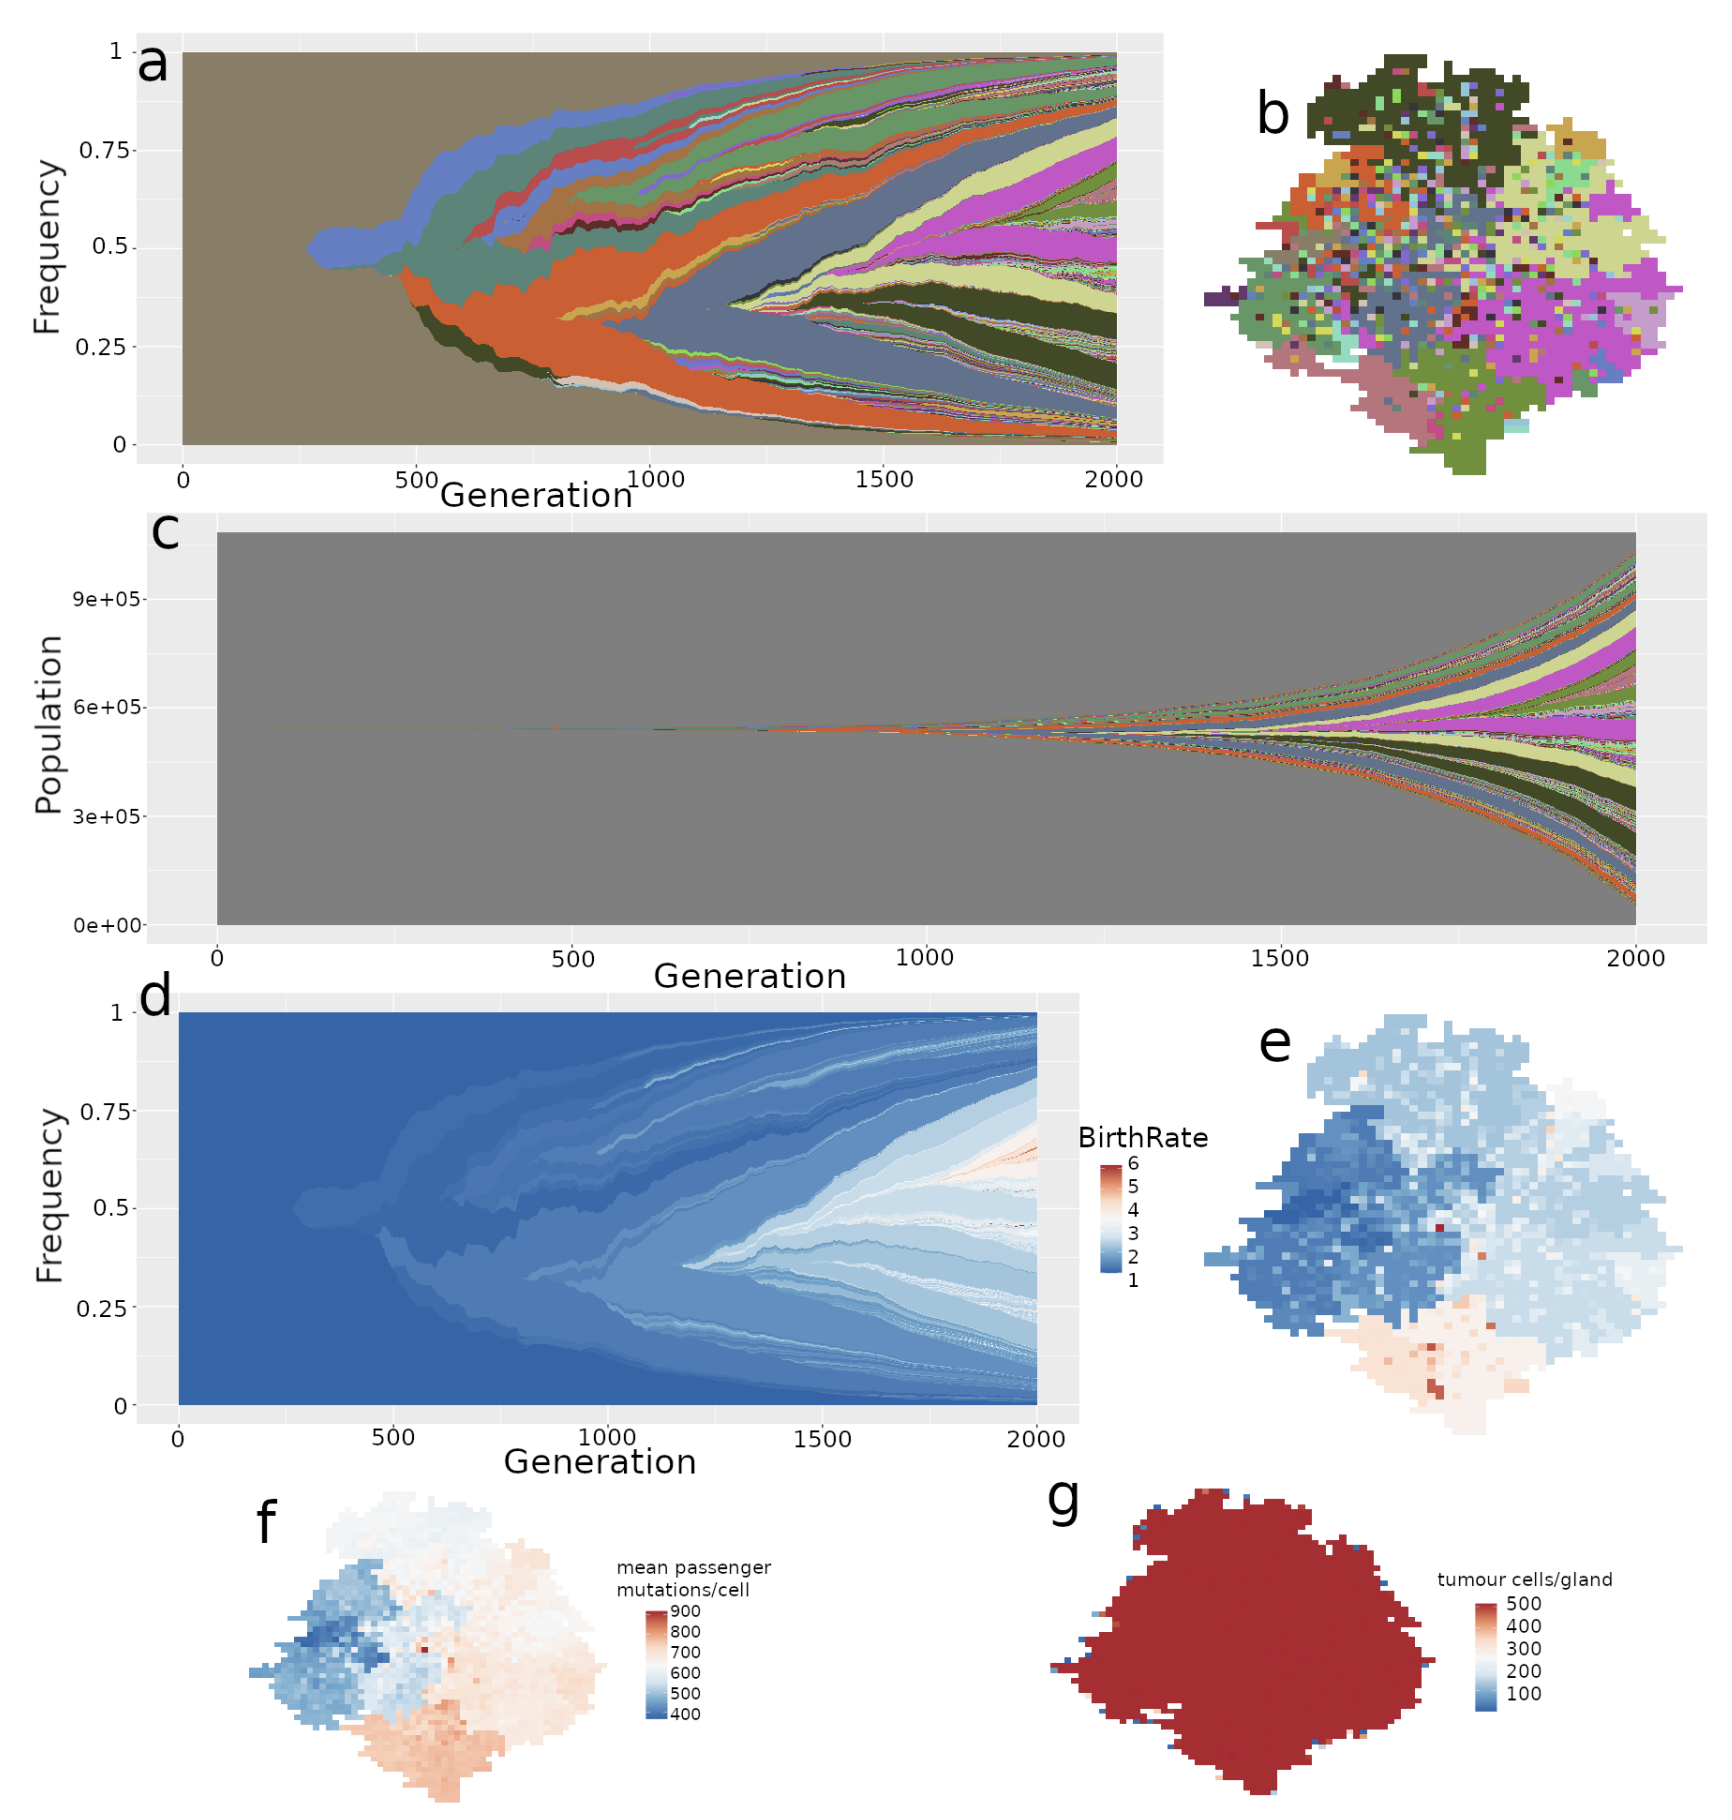
\includegraphics[width=\textwidth]{Chapter_1/figures/demonanalysis_example.png}
    \caption{Example output from \texttt{demon}, visualised using the \texttt{demonanalysis} package.}
    \label{fig:demonanalysis_example}
\end{figure}

\section{Likelihood-free inference}
\subsection{Introduction}
\textit{General introduction to Bayesian inference and the need for likelihood-free methods.}

\subsection{Approximate Bayesian Computation}
\textit{Background on ABC and its use in cancer research.}

\section{Fluctuating methylation clocks}
